\RequirePackage{plautopatch}
\documentclass[13pt,aspectratio=169,table,dvipdfmx]{beamer}

\usepackage{animate}
\usepackage{bxdpx-beamer}
\usepackage{amsmath, amssymb, amsthm, mathrsfs, amsfonts, dsfont}
\usepackage[linesnumbered, ruled, vlined]{algorithm2e}
\usepackage{annotate-equations}
\usepackage{bbm}
\usepackage{bm}
\usepackage{booktabs}
\usepackage{breakcites}
\usepackage{calc}
\usepackage[style=base]{caption}
\usepackage{enumerate}
\usepackage[T1]{fontenc}
\usepackage{ifthen}
\usepackage{listings}
\usepackage{mathtools}
\usepackage{makecell}
\usepackage{mlmodern}
\usepackage{multirow}
\usepackage{newtxtext}
\usepackage{optidef}
\usepackage[deluxe]{otf}
\usepackage{physics}
\usepackage{pifont}
\usepackage{setspace}
\usepackage{stfloats}
\usepackage{subfiles}
\usepackage{subcaption}
\usepackage{svg}
\usepackage{tikz}
\usepackage{xparse}
\usepackage[all]{xy}

% === Commands ===

\definecolor{cA}{HTML}{0072BD}
\definecolor{cB}{HTML}{EDB120}
\definecolor{cC}{HTML}{77AC30}
\definecolor{cD}{HTML}{D95319}
\definecolor{cE}{HTML}{7E2F8E}
\newcommand{\cAText}[1]{\textcolor{cA}{#1}}
\newcommand{\cBText}[1]{\textcolor{cB}{#1}}
\newcommand{\cCText}[1]{\textcolor{cC}{#1}}
\newcommand{\cDText}[1]{\textcolor{cD}{#1}}
\newcommand{\cEText}[1]{\textcolor{cE}{#1}}
\newcommand{\red}[1]{\textcolor{red}{#1}}
\newcommand{\blue}[1]{\textcolor{blue}{#1}}
\newcommand{\green}[1]{\textcolor{green}{#1}}
\newcommand{\gray}[1]{\textcolor{gray}{#1}}
\newcommand{\black}[1]{\textcolor{black}{#1}}

\newcommand{\st}{\text{ s.t. }}
\newcommand{\Img}[1]{\mathrm{Im}\qty(#1)}
\newcommand{\Ker}[1]{\mathrm{Ker}\qty(#1)}
\newcommand{\Supp}[1]{\mathrm{supp}\qty(#1)}
\newcommand{\Rank}[1]{\mathrm{rank}\qty(#1)}
\newcommand{\floor}[1]{\left\lfloor #1 \right\rfloor}
\newcommand{\ceil}[1]{\left\lceil #1 \right\rceil}
% C++ (https://tex.stackexchange.com/questions/4302/prettiest-way-to-typeset-c-cplusplus)
\newcommand{\Cpp}{C\nolinebreak[4]\hspace{-.05em}\raisebox{.4ex}{\relsize{-3}{\textbf{++}}}}
% https://tex.stackexchange.com/questions/28836/typesetting-the-define-equals-symbol
\newcommand{\defeq}{\coloneqq}
\newcommand{\eqdef}{\eqqcolon}
% https://tex.stackexchange.com/questions/5502/how-to-get-a-mid-binary-relation-that-grows
\newcommand{\relmiddle}[1]{\mathrel{}\middle#1\mathrel{}}
\newcommand{\cmark}{\cCText{\ding{51}}} % check mark
\newcommand{\xmark}{\cDText{\ding{55}}} % cross mark

\DeclareMathOperator{\Proj}{Proj}
\DeclareMathOperator{\Exp}{Exp}
\DeclareMathOperator{\Hess}{Hess}
\DeclareMathOperator{\Retr}{Retr}
\DeclareMathOperator{\Span}{span}
\DeclareMathOperator{\myGrad}{grad}
\renewcommand{\grad}{\myGrad}

% https://tex.stackexchange.com/questions/564216/newcommand-for-each-letter
\ExplSyntaxOn
\NewDocumentCommand{\definealphabet}{mmmm}{
\int_step_inline:nnn{`#3}{`#4}{
\cs_new_protected:cpx{#1 \char_generate:nn{##1}{11}}{
\exp_not:N #2{\char_generate:nn{##1}{11}}}}}
\ExplSyntaxOff

\definealphabet{bb}{\mathbb}{A}{Z}
\definealphabet{rm}{\mathrm}{A}{Z}
\definealphabet{cal}{\mathcal}{A}{Z}
% \definealphabet{scr}{\mathscr}{A}{Z}
\definealphabet{frak}{\mathfrak}{a}{z}
\definealphabet{frak}{\mathfrak}{A}{Z}

% === Settings ===

% https://qiita.com/rityo_masu/items/efd44bc8f9229e014237
\allowdisplaybreaks[4]

\usetikzlibrary{
  3d,
  fit,
  calc,
  math,
  matrix,
  patterns,
  backgrounds,
  arrows.meta,
  decorations.pathmorphing,
}

% This declares a command \Comment
% The argument will be surrounded by /* ... */
% https://ja.overleaf.com/learn/latex/Algorithms
\SetKwComment{Comment}{/* }{ */}

\DontPrintSemicolon

\parindent=0pt

% === Beamer Settings ===

\usetheme{Boadilla}

\usefonttheme{professionalfonts} % Be professional!

% https://tex.stackexchange.com/questions/646333/size-of-integral-symbol-in-section-header-with-mlmodern
\DeclareFontFamily{OMX}{mlmex}{}
\DeclareFontShape{OMX}{mlmex}{m}{n}{%
   <->mlmex10%
   }{} 
\renewcommand{\familydefault}{\sfdefault}
\usefonttheme{structurebold}
\setbeamerfont{alerted text}{series=\bfseries}
\setbeamerfont{section in toc}{series=\mdseries}
\setbeamerfont{itemize/enumerate body}{size=\large}

%Beamer Color
\definecolor{blendedblue}{rgb}{0.2,0.2,0.7}
\definecolor{UniBlue}{RGB}{0,150,200} 
\definecolor{UniGreen}{RGB}{0,200,150}
\definecolor{AlertOrange}{RGB}{255,76,0}
\definecolor{AlmostBlack}{RGB}{38,38,38}
\setbeamercolor{normal text}{fg=AlmostBlack}
\setbeamercolor{structure}{fg=UniBlue}
\setbeamercolor{block title}{fg=UniBlue!50!black}
\setbeamercolor{alerted text}{fg=AlertOrange}
\setbeamercolor{itemize item}{fg=black}
\setbeamercolor{itemize subitem}{fg=black}
\setbeamercolor{itemize subsubitem}{fg=black}

\setbeamertemplate{blocks}[rounded]
\useinnertheme{circles}
\setbeamertemplate{navigation symbols}{}
\setbeamertemplate{footline}[page number]

\setbeamertemplate{title page}{%
    \vspace{2.5em}
    {\usebeamerfont{title} \usebeamercolor[fg]{title} \inserttitle \par}
    {\usebeamerfont{subtitle}\usebeamercolor[fg]{subtitle}\insertsubtitle \par}
    \vspace{1.5em}
    \begin{flushright}
        \usebeamerfont{author}\insertauthor\par
        \usebeamerfont{institute}\insertinstitute \par
        \vspace{3em}
        \usebeamerfont{date}\insertdate\par
        \usebeamercolor[fg]{titlegraphic}\inserttitlegraphic
    \end{flushright}
}

% === TITLE ===
\title{\Huge{Improved Initial Placement for\\Fruchterman--Reingold Algorithm}}
\author{\Large{Hiroki Hamaguchi}}
\institute{\large{Supervisors: Prof. Akiko Takeda\\\phantom{Supervisors: }Pierre-Louis Poirion\\\phantom{Supervisors: }Andi Han}\\\phantom{Supervisors: }if ok, Prof. Naoki Marumo}
\date{2024/11/29}

\newif\ifShowHidden
\ShowHiddenfalse
% \ShowHiddentrue

\begin{document}

\ifShowHidden
    \maketitle
\fi

\begin{frame}
    \begin{figure}[htbp]
        \begin{minipage}{0.33\hsize}
            \centering
            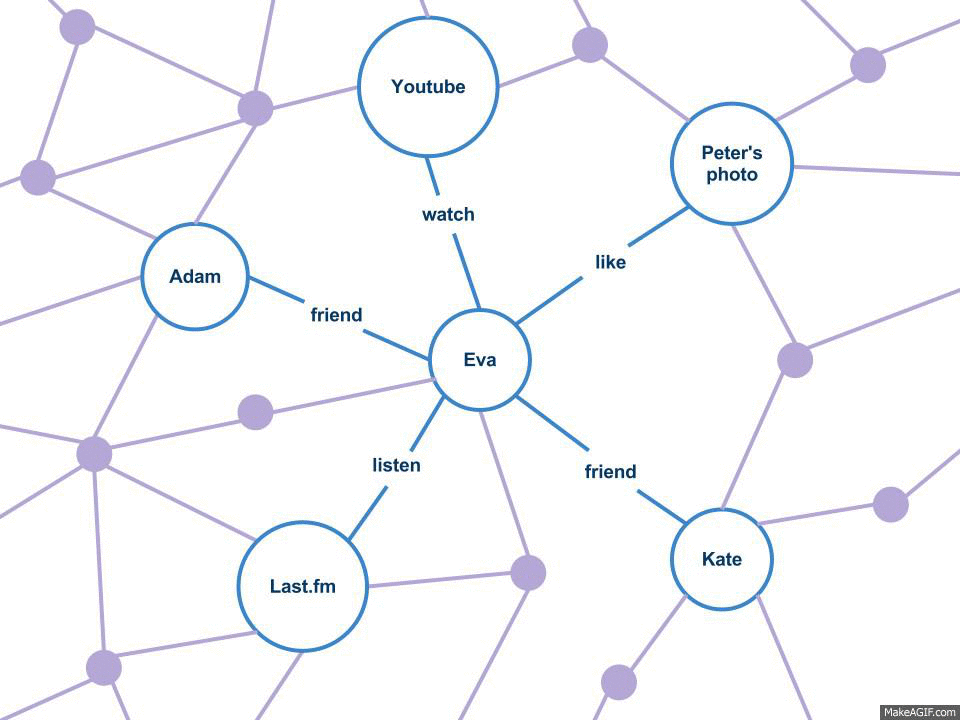
\includegraphics[width=40mm]{imgs/social_graph.png}
            \caption{
                Social Network Graph
                By \href{https://en.wikipedia.org/wiki/Social_graph#/media/File:Social_graph.gif}{Festys}, \href{https://creativecommons.org/licenses/by-sa/3.0}{CC BY-SA 3.0}, via Wikimedia Commons
            }
        \end{minipage}
        \begin{minipage}{0.33\hsize}
            \centering
            \includesvg[width=\columnwidth]{imgs/High_Speed_Railroad_Map_of_Europe.svg}
            \caption{
                Railroad Graph
                By \href{https://commons.wikimedia.org/wiki/File:High_Speed_Railroad_Map_of_Europe.svg}{Akwa and others},\href{https://creativecommons.org/licenses/by-sa/3.0}{CC BY-SA 3.0}, via Wikimedia Commons
            }
        \end{minipage}
        \begin{minipage}{0.33\hsize}
            \centering
            % \includegraphics[width=40mm]{path3.png}
            % \caption{caption3}
        \end{minipage}
    \end{figure}
\end{frame}

\ifShowHidden
    \begin{frame}{Introduction for Graph Drawing}
        \begin{tikzpicture}
            \node[cA,font=\bfseries] (A) at (0,0) {Graph Drawing};
            \node[cB] (B) at (-3.0,-1) {Discrete Based};
            \node[align=left,anchor=north west] (B1) at ($(B)+(-2.0,-0.6-0.0)$) {\cBText{BFS layout}\\\small{\quad - for tree graph}};
            \node[align=left,anchor=north west] (B2) at ($(B)+(-2.0,-0.6-1.0)$) {\cBText{Planar layout}\\\small{\quad - for planar graph}\\\scriptsize{\quad - \cite{tutteHowDrawGraph1963}}\\\scriptsize{\quad - \cite{chrobakLineartimeAlgorithmDrawing1995}}};
            \node[align=left,anchor=north west] (B3) at ($(B)+(-2.0,-0.6-3.0)$) {\cBText{Layered graph drawing}\\\small{\quad - for DAG}\\\scriptsize{\quad - \cite{sugiyamaMethodsVisualUnderstanding1981}}};
            \node[align=left,anchor=north west] (B4) at ($(B)+(-2.0,-0.6-4.5)$) {\cBText{Spectral layout~}\\\small{\quad - eigenvector of Laplacian}};
            \node[draw=cB, thick,fit={(B1) (B2) (B3) (B4)}, inner sep=5pt] (BBox) {};

            \node[cC,font=\bfseries] (C) at (+4.5,-1) {Continuous Based};
            \node[cC] (C1) at ($(C)+(-2.5,-1)$) {Kamada--Kawai (KK)};
            \node[cC] (C11) at ($(C1)+(0,-0.5)$) {\scriptsize{\cite{kamadaAlgorithmDrawingGeneral1989}}};
            \node at ($(C11)+(0,-1.0)$) {
                \begin{minipage}{4cm}
                    \begin{gather*}
                        \mathrm{minimize}\\
                        \sum_{i < j} \frac{k_{i,j}}{2} (d_{i,j}-l_{i,j})^2
                    \end{gather*}
                \end{minipage}
            };
            \node[cC,font=\bfseries] (C2) at ($(C)+(+2.5,-1)$) {Fruchterman--Reingold (FR)};
            \node[cC,font=\bfseries,align=center] (C21) at ($(C2)+(0,-0.5)$) {\scriptsize{\cite{fruchtermanGraphDrawingForcedirected1991}}};
            \node at ($(C21)+(0,-1.0)$) {
                \begin{minipage}{4cm}
                    \begin{gather*}
                        \mathrm{minimize}\\
                        \sum_{i<j} \qty(\frac{a_{i,j} d_{i,j}^3}{3k} - k^2\log{d_{i,j}})
                    \end{gather*}
                \end{minipage}
            };

            \node[align=center] (C3) at ($(C)+(0.5,-4.3)$) {
            \scriptsize{$d_{i,j}$: distance between nodes $v_i,v_j$ \;/\; $l_{i,j}$: optimal distance \;/\; $k,a_{i,j}$: constant}
            };

            \node (C01) at ($(C)+(-3.5,-5.5)$) {
                
\includegraphics[width=1cm]{imgs/networkx_logo.png}
            };
            \node (C02) at ($(C)+(-2.5,-5.5)$) {
                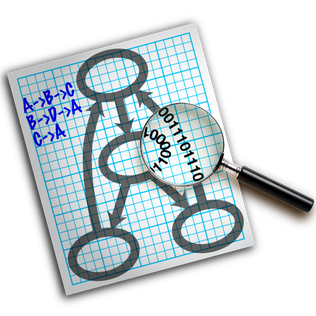
\includegraphics[width=1cm]{imgs/GraphvizLogo.png}
            };
            \node[anchor=west] (C03) at ($(C)+(-2,-5.5)$) {
                NetworkX and Graphviz support KK and FR
            };
            \node[draw=cC, thick,fit={(C01) (C02) (C03)}, inner sep=5pt] (CBox) {};

            \draw[thick,->] (A) |- ($(A)!0.5!(B)$) -| (B);
            \draw[thick,->] (A) |- ($(A)!0.5!(C)$) -| (C);
            \draw[thick,->] (C) |- ($(C)!0.5!(C1)$) -| (C1);
            \draw[thick,->] (C) |- ($(C)!0.5!(C2)$) -| (C2);
        \end{tikzpicture}
    \end{frame}
\fi

\ifShowHidden
    \begin{frame}{Definition of FR Layout}
        \begin{itemize}
            \item Historically, FR layout seeks an \textbf{equilibrium of two forces}:
        \end{itemize}
        \begin{equation*}
            F_{i,j}^a(d) \defeq \frac{a_{i,j} d^2}{k} \text{\quad (attraction)}, \quad F^r(d) \defeq -\frac{k^2}{d} \text{\quad (repulsion)}
        \end{equation*}
        \begin{itemize}
            \item This problem can be redefine as an optimization problem:
        \end{itemize}
        \begin{equation*}
            \mathrm{minimize} \; \sum_{i<j} E_{i,j}(d)
            \quad \mathrm{where} \quad
            E_{i,j}(d) \defeq \int_{0}^{d} F_{i,j}^a(r) \dd{r} + \int_{\infty}^{d} F^r(r) \dd{r} = \frac{a_{i,j} d^3}{3k} - k^2\log{d}
        \end{equation*}
        \begin{figure}[htbp]
            \begin{minipage}{0.49\hsize}
                \centering
                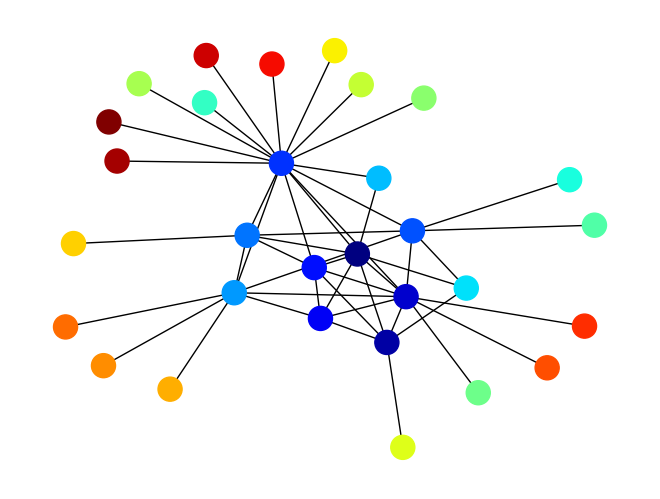
\includegraphics[width=0.6\columnwidth]{imgs/example_fr.png}
                \caption{
                    Example of FR layout
                    % 3d graph drawing \cite{doi:10.1177/14738716211060306}
                }
            \end{minipage}
            \begin{minipage}{0.49\hsize}
                \centering
                \begin{tikzpicture}
                    \def\yAdjust{2}
                    \def\d{4}
                    \def\r{0.3}
                    \def\u{1.0}
                    \coordinate (M1) at (0,0);
                    \coordinate (M2) at (\d,0);

                    \draw (M1) circle(\r) node {$v_i$};
                    \draw (M2) circle(\r) node {$v_j$};

                    \draw (0,+1.6*\r*\yAdjust) -- (0,+2.4*\r*\yAdjust);
                    \draw (\d,+1.6*\r*\yAdjust) -- (\d,+2.4*\r*\yAdjust);
                    \draw[{Latex[length=4,width=3]}-{Latex[length=4,width=3]}] ($(M1)+(90:2*\r*\yAdjust)$) -- ($(M2)+(90:2*\r*\yAdjust)$)
                    node[midway,circle,fill=white,inner sep=0] {$d = k/a_{i,j}^{1/3}$};

                    \draw[->,thick,line cap=round] (+\r,0) -- (+\u,0) node[right] {$F^a_{i,j}(d)$};
                    \draw[->,thick,line cap=round] (-\r,0) -- (-\u,0) node[left] {$F^r(d)$};

                    \draw[dashed,domain=3.9:-3.1,samples=1000,smooth,variable=\x] plot(\x,{(-0.7+(pow((\d-\x)/\d,3)/3-ln((\d-\x)/\d))/2.2)*\yAdjust});
                    \node [star,
                        minimum size=0.25cm,
                        star point ratio=2.25,
                        inner sep=0pt,
                        draw, fill=black]
                    at (0,{(-0.7+(1/3)/2.2)*\yAdjust}) {};

                    \node at (-2.7,0.4*\yAdjust) {$E_{i,j}(d)$};
                \end{tikzpicture}
            \end{minipage}
        \end{figure}
    \end{frame}
\fi

\ifShowHidden
    \begin{frame}{Algorithm for FR Layout 1}
        \begin{columns}
            \begin{column}{0.4\columnwidth}
                \textbf{``spring\_layout'' in NetworkX\\and ``fdp'' in Graphviz}
                \begin{itemize}
                    \item Adaptive cooling scheme
                    \item \textbf{gradient descent method}\\with constant step size\\per each vertex
                    \item strong \textbf{theoretical background}
                    \item \cite{tunkelang1999numerical}
                \end{itemize}
            \end{column}
            \begin{column}{0.6\columnwidth}
                \begin{figure}[htbp]
                    \centering
                    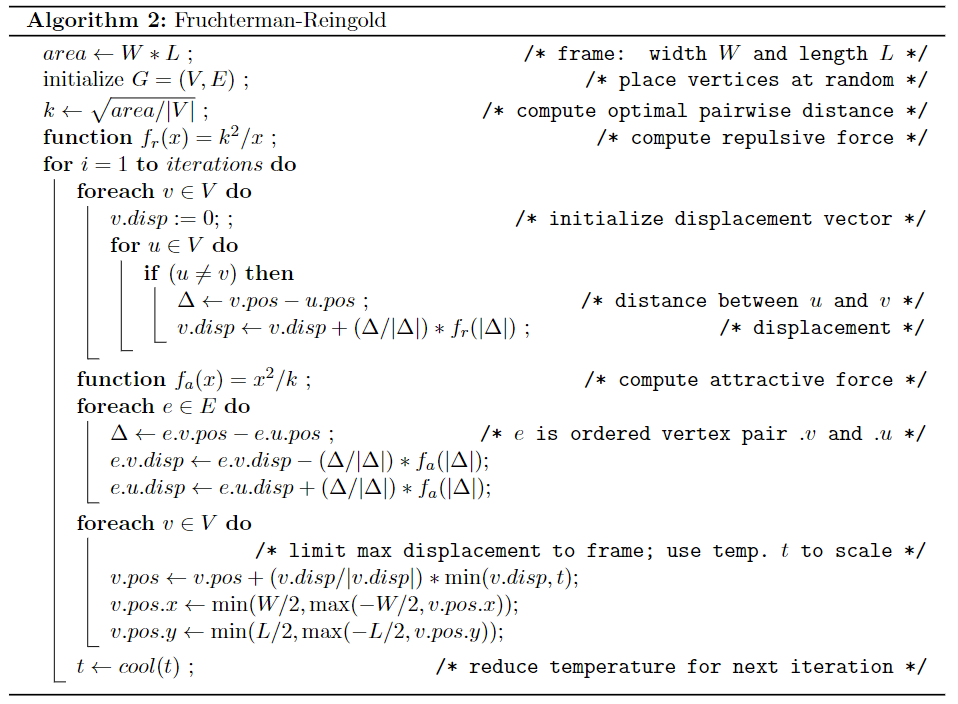
\includegraphics[width=\columnwidth]{imgs/FR_code.png}
                    \caption{\cite{kobourov2012spring}}
                \end{figure}
            \end{column}
        \end{columns}
    \end{frame}
    \begin{frame}{Algotithm for FR Layout 2}
        \begin{columns}
            \begin{column}{0.4\columnwidth}
                \textbf{``sfdp'' in Graphviz}
                \begin{itemize}
                    \item Scalable Force-Directed Placement
                    \item \textbf{Multilevel} approach
                    \item Barnes--Hut algorithm (Q-tree)\cite{Hu2006EfficientHF}
                          \cite{barnesHierarchicalLogForcecalculation1986}
                    \item These methods are\\\textbf{out of scope},\\
                          but our work is still \textbf{applicable}.
                \end{itemize}
            \end{column}
            \begin{column}{0.6\columnwidth}
                \begin{figure}[htbp]
                    \centering
                    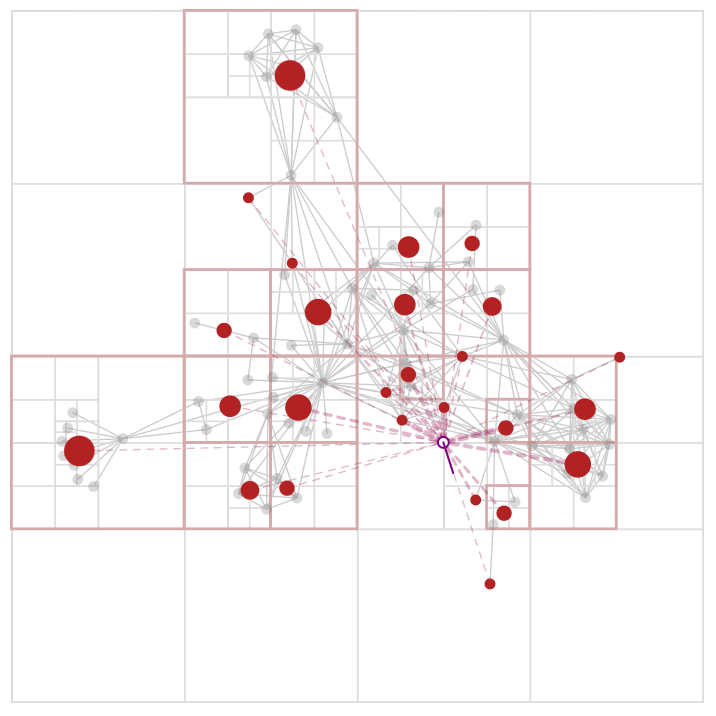
\includegraphics[width=0.7\columnwidth]{imgs/BH.png}
                    \caption{\footnotesize{\url{https://jheer.github.io/barnes-hut/}}}
                \end{figure}
            \end{column}
        \end{columns}
    \end{frame}
\fi

\ifShowHidden
    \begin{frame}{Hardness of graph drawing}
        \begin{itemize}
            \item FR algorithm is powerful for network-like graphs, but \textbf{not for other types}.
            \item Escaping from a plateau is \textbf{very difficult}.
            \item Drawing $\bigcirc$ $\cong$ untangling tangled earphones
        \end{itemize}
        \begin{figure}[htbp]
            \begin{minipage}{0.59\hsize}
                \centering
                \animategraphics[autoplay,loop,width=0.8\columnwidth]{5}{imgs/circle/circle-}{1}{50}
                % 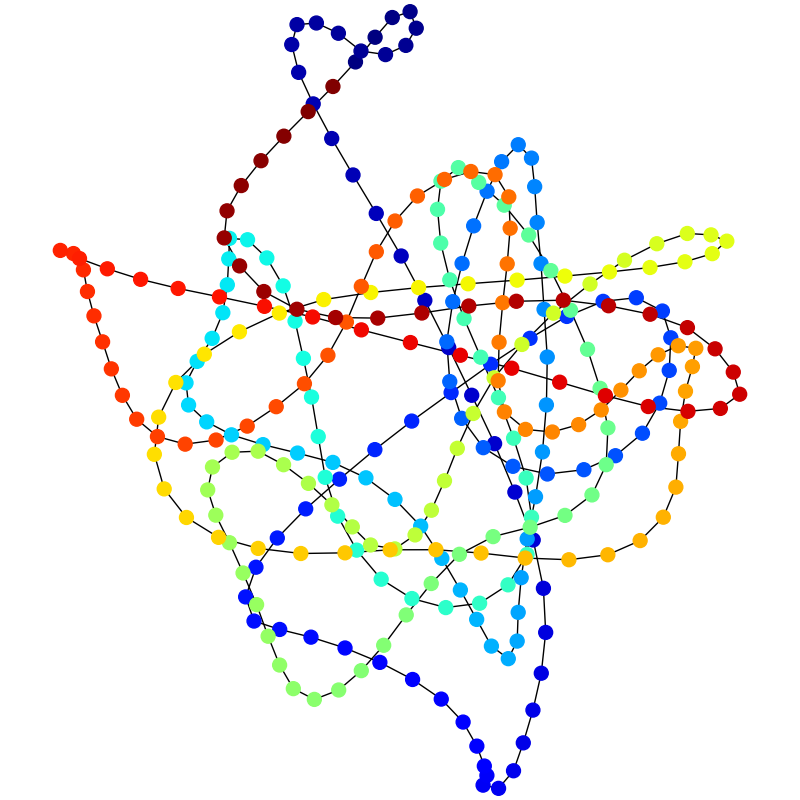
\includegraphics[width=0.8\columnwidth]{imgs/circle/circle-50.png}
                \caption{FR layout by NetworkX}
            \end{minipage}
            \begin{minipage}{0.40\hsize}
                \centering
                \includesvg[width=0.8\columnwidth]{imgs/circle_fdp.svg}
                \caption{fdp layout by Graphviz}
            \end{minipage}
        \end{figure}
    \end{frame}
\fi

\ifShowHidden
    \begin{frame}{Graph Drawing as Continuous Optimization Problem}
        \begin{itemize}
            \item Research on graph drawing by \textbf{continuous optimization} is a hot topic.
                  \begin{itemize}
                      \large{
                      \item stress majorization \cite{gansnerGraphDrawingStress2005}
                      \item \textbf{L-BFGS} method~\cite{6183577} \cEText{(8 cites)}
                      \item GPU based \cite{gajdosParallelFruchtermanReingold2016}
                      \item \textbf{SGD} (stochastic gradient descent)~\cite{8419285} \cEText{(66 cites)}
                      \item and so on \cite{ahmedGraphDrawingGradient2020,ahmedMulticriteriaScalableGraph2022,khanManyobjectiveEvolutionaryAlgorithm2024}
                            }
                  \end{itemize}
        \end{itemize}
        \begin{center}
            \textcolor{gray}{todo: explanation of L-BFGS and SGD\\
                L-BFGs: quasi-Newton method with limited memory\\
                SGD: stochastic gradient descent (mini-batch)}
        \end{center}
        $\to$ Our research aims to take over this flow of the research.
    \end{frame}
\fi

\ifShowHidden
    \begin{frame}{Problem: Inapplicability of SGD}
        \begin{itemize}
            \item \textbf{SGD} is powerful for KK layout, but \textbf{not for FR layout}.
            \item KK layout first computes the optimal distance $l_{i,j}$ by Dijkstra's algorithm.
            \item FR layout has $a_{i,j}=0$ if $v_i,v_j$ are not connected.
        \end{itemize}
        \begin{columns}
            \begin{column}{0.1\columnwidth}\end{column}
            \begin{column}{0.4\columnwidth}
                \begin{equation*}
                    \mathrm{(KK)} \quad  f_{i,j}(d) = \frac{k}{2} (d_{i,j} - l_{i,j})^2
                \end{equation*}
            \end{column}
            \begin{column}{0.4\columnwidth}
                \begin{equation*}
                    \mathrm{(FR)} \quad  f_{i,j}(d) = \frac{a_{i,j} d^3}{3k} - k^2\log{d}
                \end{equation*}
            \end{column}
            \begin{column}{0.1\columnwidth}\end{column}
        \end{columns}
        \begin{figure}[htbp]
            \centering
            \begin{tikzpicture}
                \def\radius{2}
                \foreach \xShift/\nA/\nB/\nC/\nD/\nE/\nF/\desc in {
                        -3/1/2/3/3/2/1/$l_{i,j}$,
                        +3/1/0/0/0/0/1/$a_{i,j}$} {
                        \begin{scope}[xshift=\xShift cm]
                            \node at (-0.85*\radius,+0.85*\radius) {\large{\desc}};
                            \node (P0) at (0:\radius) [circle, fill=red, inner sep=0pt, minimum size=10pt] {};
                            \foreach \i in {1,...,6} {
                                    \node (P\i) at (\i*360/7: \radius) [circle, fill=black, inner sep=0pt, minimum size=6pt] {};
                                }
                            \draw (P0) -- (P1) -- (P2) -- (P3) -- (P4) -- (P5) -- (P6) -- (P0);
                            \foreach \i in {1,...,6} {
                                    \draw [decorate, decoration={coil,aspect=0.6,segment length=2mm,amplitude=1mm}] (P\i) -- (P0);
                                }
                            \node[right=5pt] at ($(P0)!0.5!(P1)$) {\nA};
                            \node[above=5pt] at ($(P0)!0.5!(P2)$) {\nB};
                            \node[above=5pt] at ($(P0)!0.5!(P3)$) {\nC};
                            \node[below=5pt] at ($(P0)!0.5!(P4)$) {\nD};
                            \node[below=5pt] at ($(P0)!0.5!(P5)$) {\nE};
                            \node[right=5pt] at ($(P0)!0.5!(P6)$) {\nF};
                        \end{scope}
                    }
            \end{tikzpicture}
        \end{figure}
    \end{frame}
\fi

% \ifShowHidden
\begin{frame}{The Purpose of this research}
    \begin{table}
        \centering
        \begin{tabular}{c|c|c|c}
            \toprule
            Existing works                       & \makecell[c]{\cite{6183577}                                                                                         \\\cite{8419285}}    & \cite{ghassemitoosiSimulatedAnnealingPreProcessing2016} & \cite{NEURIPS2019_bc6dc48b}           \\
            \midrule
            \textbf{abstract}                    & \makecell[c]{L-BFGS / SGD                                                                                           \\for graph drawing} & \makecell[c]{pre-processing as\\initial placement}                     & \makecell[c]{random subspace\\algorithm}             \\[1.5em]
            \textbf{limitation}                  & \makecell[c]{L-BFGS is slow                                                                                         \\SGD is un-apllicable} & \makecell[c]{just using\\a circle layout}                     & \makecell[c]{no existing work\\for FR layout}             \\
            \midrule
            \textcolor{red}{\textbf{What we do}} & \textcolor{red}{practical speed up} & \textcolor{red}{refine the strategy} & \makecell[c]{\textcolor{red}{apply to} \\\textcolor{red}{FR layout}} \\
            \bottomrule
        \end{tabular}
    \end{table}
\end{frame}
% \fi

\ifShowHidden
    \begin{frame}{Key Observation: stochastic strategy}
        \begin{columns}
            \begin{column}{0.49\columnwidth}
                \centering{
                    For far-quadratic objective functions
                    \begin{itemize}
                        \item[\cmark] \textbf{SGD} excels at rough optimization
                        \item[\xmark] \textbf{L-BFGS} is ineffective for this case\\
                            \small{$\order{\abs{V}^2}$ per iteration is too expensive}
                    \end{itemize}}
            \end{column}
            \begin{column}{0.49\columnwidth}
                \centering{
                    For near-quadratic objective functions
                    \begin{itemize}
                        \item[\cmark] \textbf{L-BFGS} excels at precise optimization
                        \item[\xmark] \textbf{SGD} is ineffective for this case\\
                            \small{it is too easy to find a locally optimal solution}
                    \end{itemize}}
            \end{column}
        \end{columns}
        \begin{figure}[htbp]
            \centering
            \begin{tikzpicture}
                \foreach \xA/\yA/\xB/\yB/\xC/\yC/\xD/\yD/\xE/\yE/\xShift/\yShift in {
                        1.25/1.25/-0.25/0.75/-0.25/-1.25/0.75/-0.25/-1.25/-0.25/-5/0,
                        0/0/0/1/0/-1/1/0/-1/0/0/0,
                        0.2/-0.1/-0.3/1.2/-0.2/-0.9/1.1/-0.1/-1.1/0.1/+5/0} {
                        \begin{scope}[xshift=\xShift cm,yshift=\yShift cm]
                            \draw[dashed,color=gray,line width=0.5pt] (-1.5, 1.5) rectangle (1.5, -1.5);
                            \node[circle, fill=red,   minimum size=8pt] (a0) at (\xA, \yA) {};
                            \node[circle, fill=black, minimum size=8pt] (a1) at (\xB, \yB) {};
                            \node[circle, fill=black, minimum size=8pt] (a2) at (\xC, \yC) {};
                            \node[circle, fill=black, minimum size=8pt] (a3) at (\xD, \yD) {};
                            \node[circle, fill=black, minimum size=8pt] (a4) at (\xE, \yE) {};
                            \draw[decorate, decoration={coil, segment length=2, aspect=0.5}] (a0) -- (a1);
                            \draw[decorate, decoration={coil, segment length=2, aspect=0.5}] (a0) -- (a2);
                            \draw[decorate, decoration={coil, segment length=2, aspect=0.5}] (a0) -- (a3);
                            \draw[decorate, decoration={coil, segment length=2, aspect=0.5}] (a0) -- (a4);
                        \end{scope}
                    }

                \draw[-{Latex[length=10,width=0.4cm]},line width=0.15cm] (-3.1, 0) -- (-1.9, 0);
                \draw[-{Latex[length=10,width=0.4cm]},line width=0.15cm] (+3.1, 0) -- (+1.9, 0);
            \end{tikzpicture}
        \end{figure}
    \end{frame}
\fi

\ifShowHidden
    \begin{frame}{Key Technique 1: Separation of the objective function}
        \begin{align*}
            f(X) =                      & \sum_{i<j} f_{i,j}(d_{i,j}) = \cAText{\overset{\text{attraction}}{\underbrace{\sum_{(i,j)\in E} f^a_{i,j}(d_{i,j})}_{\text{sparse}}}} + \cDText{\overset{\text{repulsion}}{\underbrace{\sum_{i<j} f^r_{i,j}(d_{i,j})}_{\text{dense}}}} \\
            \to \mathrm{minimize} \quad & \cAText{\sum_{(i,j)\in E} f^a_{i,j}(d_{i,j})} \quad \mathrm{subject \enspace to} \quad \cDText{f^r_{i,j}(d_{i,j}) \leq \epsilon, \quad i<j}                                                                                            \\
            \to \mathrm{minimize} \quad & \cAText{\sum_{(i,j)\in E} f^a_{i,j}(d_{i,j})} \quad \mathrm{subject \enspace to} \quad \cDText{\text{each $x_i$ has an exclusive $\epsilon'$-ball}}
        \end{align*}
        \begin{itemize}
            \item Without constraints, $X=0$ is the optimal solution $\to$ \textbf{closest packing}
            \item With \textbf{hexagonal close-packed} structure,
                  $f$ is the sum of $\abs{V}^2 \to \abs{E}$ terms
            \item partially overlapped with \cite{ghassemitoosiSimulatedAnnealingPreProcessing2016,s22145179}
        \end{itemize}
    \end{frame}
\fi

\begin{frame}{proposed algorithm 1}
    \begin{itemize}
        \item exact projection: min cost flow problem $(\order{\abs{V}^3})$
        \item heuristic projection: sort by coordinates $(\order{\abs{V} \log \abs{V}})$
    \end{itemize}
    \begin{figure}[htbp]
        \begin{minipage}{0.45\hsize}
            \centering
            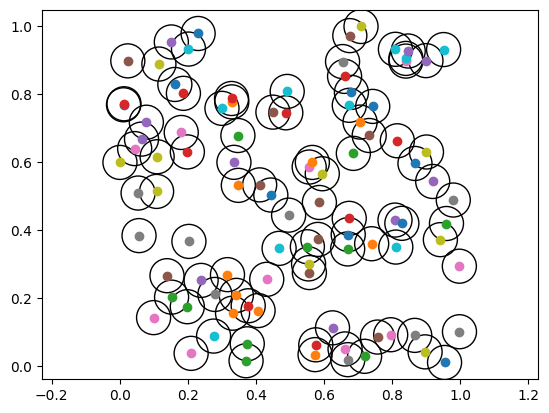
\includegraphics[width=\columnwidth]{imgs/hex1.png}
        \end{minipage}
        \begin{minipage}{0.45\hsize}
            \centering
            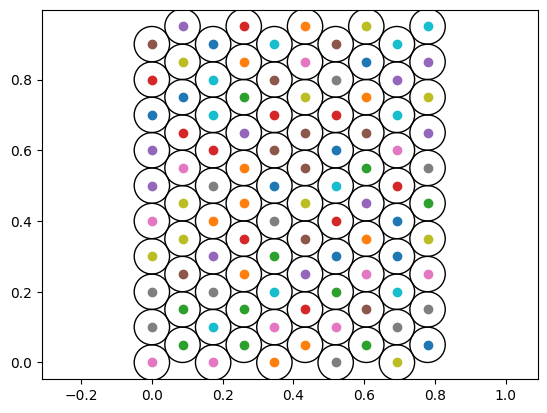
\includegraphics[width=\columnwidth]{imgs/hex2.png}
        \end{minipage}
    \end{figure}
\end{frame}

\ifShowHidden
    \begin{frame}{\cEText{余談: TSPとの関連性}}
        \begin{itemize}
            \item 固定された頂点配置に対して、サイクルグラフの頂点の割り当てを考える
            \item 最小化すべき関数$f^a(d)$を、FRレイアウトに限らず一般化して考える
            \item 特に、$f^a(d)=d$とした時、これはTSPに他ならない
            \item TSPは当然NP困難 ヒューリスティックによって解かれる
                  \begin{itemize}
                      \item 代表的なTSPの解法: (Held-Karp), 2-opt, 3-opt, Lin-Kernighan, Christofides, etc.
                      \item 参考になる部分とならない部分がそれぞれある。
                  \end{itemize}
            \item 面白い関連性として挙げてみました
        \end{itemize}
    \end{frame}
\fi

\ifShowHidden
    \begin{frame}{Key Technique 2: Randomized subspace algorithm}
        \begin{itemize}
            \item Researches on Randomized Subspace Newton (\textbf{RSN}) are conducted.
                  \begin{itemize}
                      \item Proposed in~\cite{NEURIPS2019_bc6dc48b}
                      \item Extended in~\cite{cartisRandomisedSubspaceMethods2022},\cite{fujiRandomizedSubspaceRegularized2022},\cite{higuchiFastConvergenceSecondOrder2024}
                      \item Analysis is based on~\cite{karimireddyGlobalLinearConvergence2018}
                  \end{itemize}
        \end{itemize}
        \begin{columns}[T]
            \column{0.5\columnwidth}
            \begin{itemize}
                \item Apply some second-order method to subspaces
                \item graph drawing: optimize over $\prod_{i=1}^{n} \mathbb{R}^2$\\
                      $\to$ suitable for \textbf{RSN}!
            \end{itemize}
            \column{0.5\columnwidth}
            \begin{figure}[htbp]
                \centering
                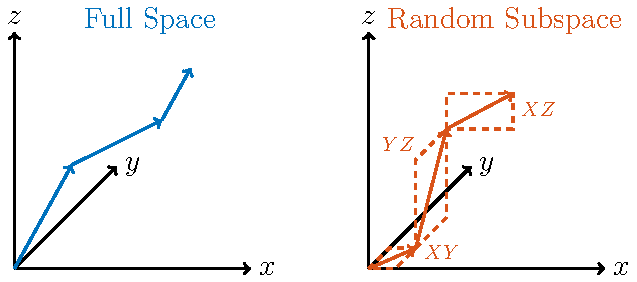
\includegraphics[width=0.9\columnwidth]{imgs/randomSubspace.pdf}
            \end{figure}
        \end{columns}
    \end{frame}
\fi

% \ifShowHidden
\begin{frame}{Advantages of Randomized Subspace Newton}
    \begin{figure}[htbp]
        \centering
        \begin{tikzpicture}[scale=1.5]
            \coordinate (A) at (0,0);
            \coordinate (B) at (3,0);
            \coordinate (C) at (0,2);

            \draw[decorate, decoration={coil, segment length=4, aspect=0.5}] (A) -- (B);
            \draw[decorate, decoration={coil, segment length=4, aspect=0.5}] (A) -- (C);

            \draw[gray, dashed, ultra thick] (A) -- ++(9/2.8,4/2.8);
            \draw[red, ultra thick, -] (A) -- ++(1.125,0.57142);
            \node[star, star points=5, star point ratio=2.25, fill=red,scale=0.5] at ($(A)+(1.125,0.57142)$) {};
            \node[anchor=west,align=left,gray] at ($(A)+(9/2.8+0.3,4/2.8)$) {\Large{$g=\nabla f$}\\[0.4em]\Large{Descent direction}};
            \node[anchor=west,align=left,red] at (9/2.8+0.3,0.5) {\Large{$d=(\nabla^2 f)^{-1}\nabla f$}\\[0.4em]\Large{Newton's direction}};

            \coordinate (opt) at ($(B)!0.5!(C)$);
            \node[star, star points=5, star point ratio=2.25, fill=cA, minimum size=5pt] at (opt) {};
            \node[above=0.5cm] at (opt) {\large{\cAText{optimal}}};

            \filldraw[red] (A) circle (2pt);
            \filldraw[black] (B) circle (2pt);
            \filldraw[black] (C) circle (2pt);
        \end{tikzpicture}
    \end{figure}
    \begin{itemize}
        \item random subspace problem (subproblem for vertex $i$):
              \begin{equation*}
                  \min_{x_i \in \mathbb{R}^2} \sum_{j \in \mathrm{Adj}(i)} \frac{a_{i,j} \norm{x_i - x_j}_2^3}{3k} \quad \leftarrow \text{\textbf{CONVEX} optimization}
              \end{equation*}
        \item Original problem, subspace problem, and restricted problem are all \textbf{NON-CONVEX}
        \item All distance $d_{i,j}=\norm{x_i-x_j}_2 \geq \epsilon'$ $\to$ numerically stable
    \end{itemize}
\end{frame}
% \fi

\ifShowHidden
    \begin{frame}{proposed algorithm 2}
        \begin{algorithm}[H]
            \SetAlgoLined
            \KwIn{Set of indices $S$, initial vectors $v_i$}
            \KwOut{Updated vector $v_i$}
            Initialize $X$ randomly\;
            \While{not converged}{
                Randomly select an index $i \in S$ except for the taboo list\;
                Compute Newton's direction $d_i=(\nabla^2 f_i)^{-1}\nabla f_i$\;
                Update $v_i$ subject to the constraints\;
                \If{not updated}{
                    Add $i$ to the taboo list\;
                }
            }
            \Return $X$\;
            \caption{Randomized Newton Direction Update for Vector $v_i$}
        \end{algorithm}
    \end{frame}
\fi

\ifShowHidden
    \begin{frame}{Possible Application 1}
        \begin{itemize}
            \item Originally, this kind of problems are solved by \textbf{stochastic coordinate descent}
            \item Random subspace algorithms might be applicable to these problems
        \end{itemize}
        \begin{figure}[htbp]
            \begin{minipage}{0.45\hsize}
                \centering
                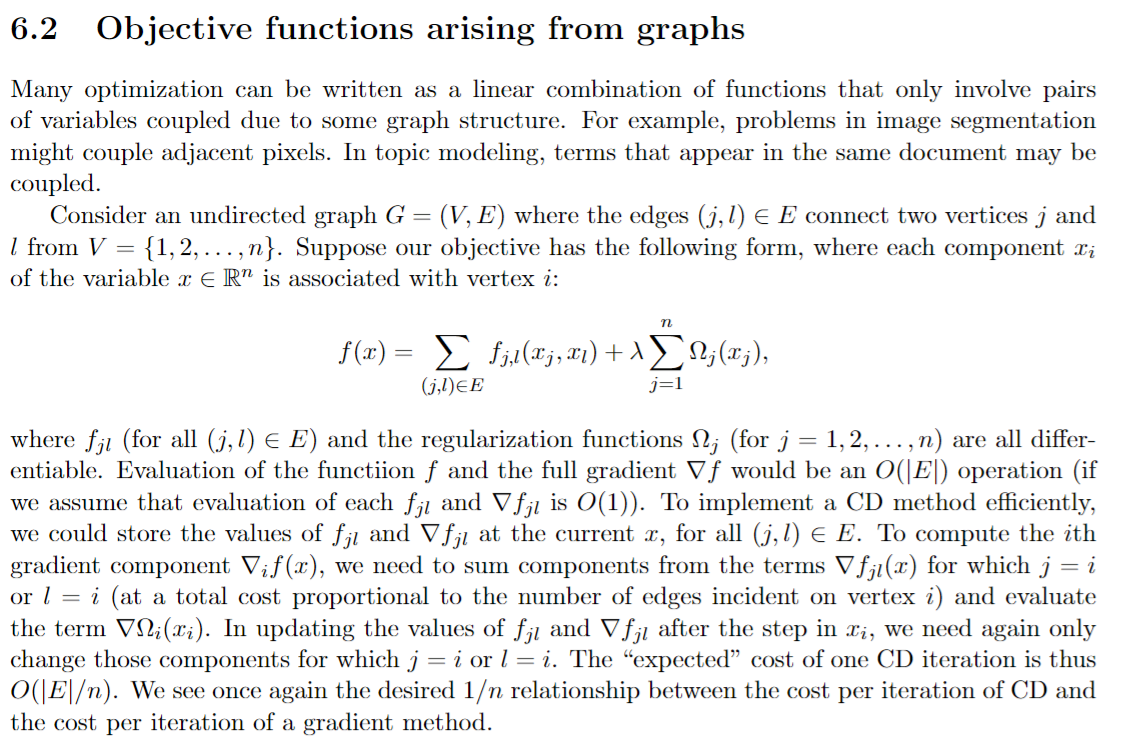
\includegraphics[width=\columnwidth]{imgs/SCD1.png}
                \caption{\href{https://people.eecs.berkeley.edu/~brecht/opt4ml_book/O4MD_06_Coordinate_Descent.pdf}{hyperlink}}
            \end{minipage}
            \begin{minipage}{0.45\hsize}
                \centering
                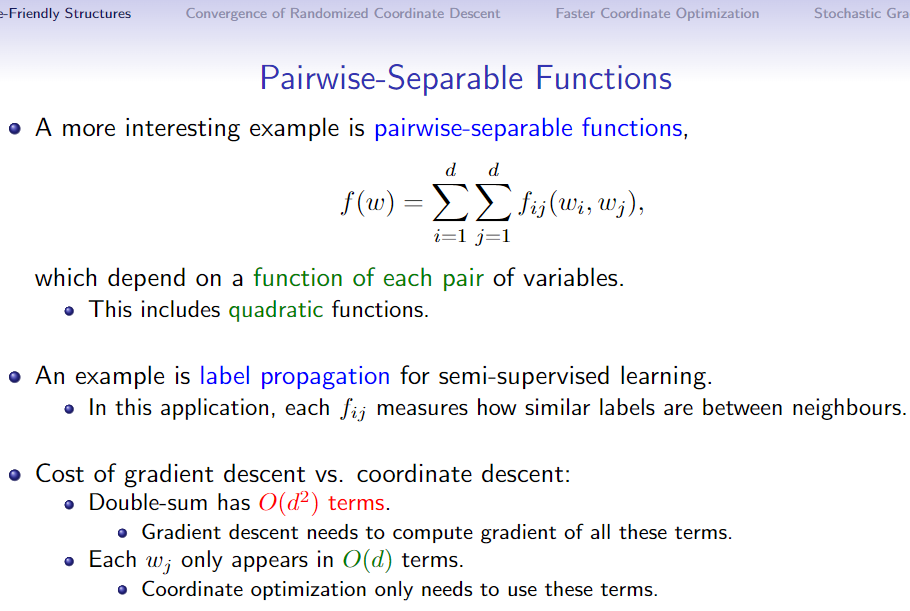
\includegraphics[width=\columnwidth]{imgs/SCD2.png}
                \caption{\href{https://www.cs.ubc.ca/~schmidtm/Courses/5XX-S22/S3.pdf}{hyperlink}}
            \end{minipage}
        \end{figure}
    \end{frame}
    \begin{frame}{Possible Application 2}
        \begin{itemize}
            \item Optimize $f(x)$ where $x \in \mathbb{R}^{n}$, not $\prod_{i=1}^{n} \mathbb{R}^2$.
            \item Assume that if two of the points are too close, $f(x)$ drastically increases.
            \item Similar algorithms might be applicable to this problem.
            \item Is there any concrete instance?
            \item Is there any algorithm already well known?
        \end{itemize}
        \begin{figure}[htbp]
            \centering
            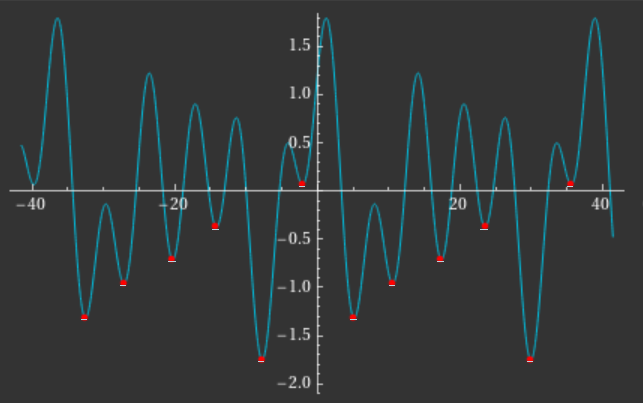
\includegraphics[width=0.5\columnwidth]{imgs/applicatoin1d.png}
        \end{figure}
    \end{frame}
    \begin{frame}{Possible Application 3}
        \begin{itemize}
            \item (Continuous relaxation of) graph isomorphism problem
                  \begin{itemize}
                      \item displaying symmetry is at least as difficult as graph isomorphism \cite{eades1984heuristic}
                      \item When we draw $G \defeq G_1 \cup G_2$, $G$ displays symmetry if $G_1 \cong G_2$.
                  \end{itemize}
            \item Graph isomorphism problem with Frank-Wolfe algorithm \cite{klusContinuousOptimizationMethods2023}
                  \begin{mini*}
                      {Q}{||QA-BQ||^2_F}{}{}
                      \addConstraint{Q}{\in \left\{ Q \in \mathbb{R}^{n \times n} \relmiddle| Q^\top Q = I_n \right\}}
                  \end{mini*}
            \item Many-to-Many graph isomorphism \cite{zaslavskiyManytoManyGraphMatching2010}
                  \begin{mini*}
                      {P}{||G - PHP^\top ||^2_F}{}{}
                      \addConstraint{P}{\in \left\{ P \in \{0, 1\}^{n \times n} \relmiddle| P1_n = 1_n, P^\top 1_n = 1_n \right\}}
                  \end{mini*}
                  % \item I'm still doubtful, but these papers seems really interesting. (+ Riemannian optimization)
            \item \cEText{(随分な遠回りでしたが、Random subspace+Riemannian optimization\\という当初の目標への回帰?)}
        \end{itemize}
    \end{frame}
\fi

\setbeamercolor{structure}{fg=blendedblue}
\setbeamercolor{block title}{fg=blendedblue!50!black}

\ifShowHidden
    \begin{frame}{Summary}
        \begin{block}{Future Work}
            \begin{itemize}
                \item More numerical experiments
                \item Theoretical analysis
            \end{itemize}
        \end{block}
    \end{frame}
\fi


% \ifShowHidden
\begin{frame}[allowframebreaks]{Reference}
    \scriptsize
    \beamertemplatetextbibitems
    \bibliographystyle{hapalike}
    \bibliography{../FruchtermanReingoldByRandomSubspace.bib}
    % \begin{thebibliography}{1}
    % \end{thebibliography}
\end{frame}
% \fi

\end{document}